% (C) Marc Lijour, 2016-2017 
% Licensed under a Creative Commons License BY-SA
% https://creativecommons.org/licenses/by-sa/2.5/ca/
% Presentation for the Small Business Digitization Initiative (SBDI) training program
% see http://www.ictc-ctic.ca/small-business-digitization-initiative/ 
% authored by Marc Lijour, December 2016
% for the session running from January 2017 to September 2017
% 
% ======================================================================================================
%                                4th INDUSTRIAL REVOLUTION
% ======================================================================================================
\section{The 4$^{th}$ Industrial Revolution}
% --------------------- Symptoms \& Drivers of the Revolution --------------------------
\subsection{Symptoms}
\begin{frame}
	\frametitle{The 4$^{th}$ Industrial Revolution}
	\framesubtitle{Everyone talks about it -Businesses \& Government alike}
	\begin{figure}
		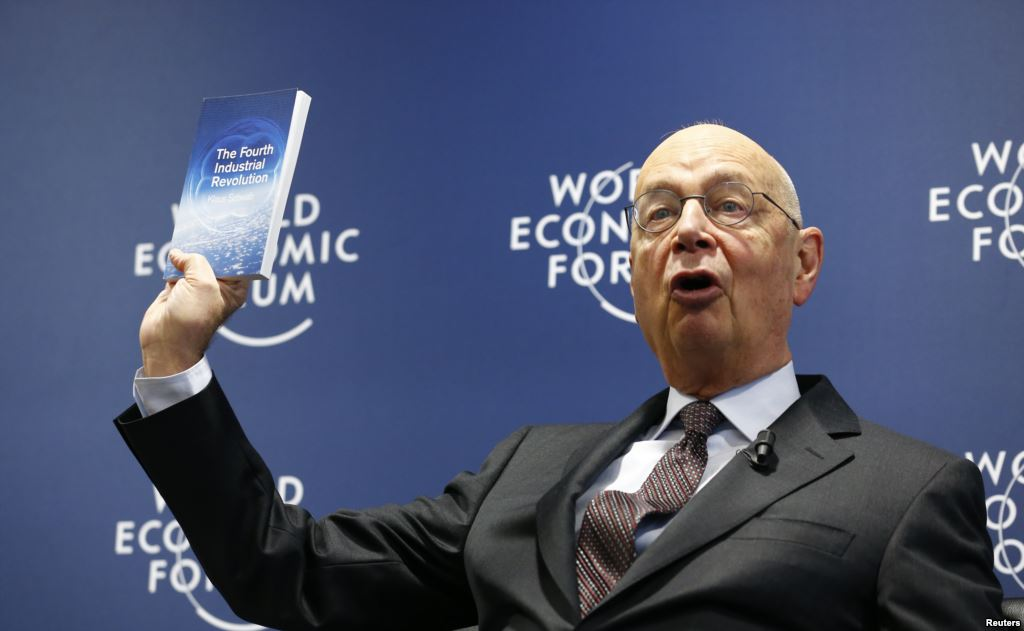
\includegraphics[width=11cm]{../pics/Schwab-4th-revolution-book-cover}
		\caption{The topic of conversation since Davos~2016 (Credit: \href{http://www.voanews.com/a/wef-founder-world-unprepared-to-deal-with-fourth-industrial-revolution/3143406.html}{Reuters})}
	\end{figure}
\end{frame}

\frame{
	\frametitle{The 4$^{th}$ Industrial Revolution}
	\framesubtitle{}
	\begin{block}{}
%		\begin{quote}
		``The new technology revolution, which entails nothing less than a transformation of mankind.'' ---Klaus Schwab, founder and executive chairman of the World Economic Forum
%		\end{quote}
	\end{block}
	\vspace{2cm}
	\fullcite{schwab2016}

}

\frame{
	\frametitle{The 4$^{th}$ Industrial Revolution}
	\framesubtitle{Characteristics}
	According to Klaus Schwab, the ``changes are historic'' because of their
	\begin{itemize}
		\item \textbf{Velocity}: Moving at an exponential pace (vs. linear) as a result of an interconnected world
		\item \textbf{Breadth \& Depth}: Touches all industries, not only technology (the \emph{what}) but also \emph{who} we are
		\item \textbf{Systems Impact}: Everything is intertwinned, and systems changes: countries, organizations, societies
	\end{itemize}
%	\begin{table}
%	\begin{tabular}{l|l}
%		Velocity 		& Moving at an exponential pace (vs. linear) as a result of an interconnected world\\
%		Breadth \& Depth 	& Touches all industries, not only technology (the \emph{what}) but also \emph{who} we are\\
%		Systems Impact		& Everything is intertwinned, and systems changes: countries, organizations, societies\\
%	\end{tabular}
%	\end{table}
}

\frame{
	\frametitle{The 4$^{th}$ Industrial Revolution}
	\framesubtitle{Technology-driven revolutions}
	\begin{itemize}
		\item \textbf{Farming} led to better food supply and the rise of urbanization
		\item The \textbf{Steam Engine} led to the 1$^{st}$ Industrial Revolution (rails roads, mechanized factories)
		\item \textbf{Electricity} led to the 2$^{nd}$ Industrial Revolution (assembly lines, mass production)
		\item \textbf{Semiconductors and Computing} led to the 3$^{rd}$ Industrial Revolution (software, the Internet)
		\item Ubiquitous Computing (cheap sensors, chips, etc), AI, and IoT are leading us through the 4$^{th}$ Industrial Revolution
	\end{itemize}
}

\frame{
	\frametitle{The 4$^{th}$ Industrial Revolution}
	\framesubtitle{The cost drivers}
	\begin{figure}
	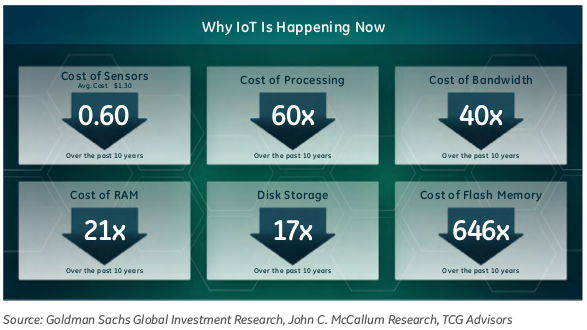
\includegraphics[width=11cm]{../pics/GE-Why-IoT-now}
	\caption{Credit: \href{http://go.digital.ge.com/IIOT-unlocking-business-value.html}{GE White Paper ``Unlocking Business Value through Industrial Data Management''}}
	\end{figure}
}

\frame{
	\frametitle{The 4$^{th}$ Industrial Revolution}
	\framesubtitle{The pace of change}
	\begin{itemize}
		\item The iPhone is only 10 years old (2007)
		\item There were 2 billion smartphones at the end of 2015
	\end{itemize}
}

\frame{
	\frametitle{The 4$^{th}$ Industrial Revolution}
	\framesubtitle{Exercise}
	\begin{alertblock}{Group Work}
		What are the new technologies that can disrupt the way we live and work?
	\end{alertblock}
}
% --------------------- Industry Positioning (Strategy, Actions) --------------------------
\subsection{Industry Positioning}
% Case studies and White papers from Cisco, GE.. 
% Videos from Davos.. 
\frame{
	\frametitle{The 4$^{th}$ Industrial Revolution}
	\framesubtitle{Technology Drivers (Networking)}
	\begin{figure}
	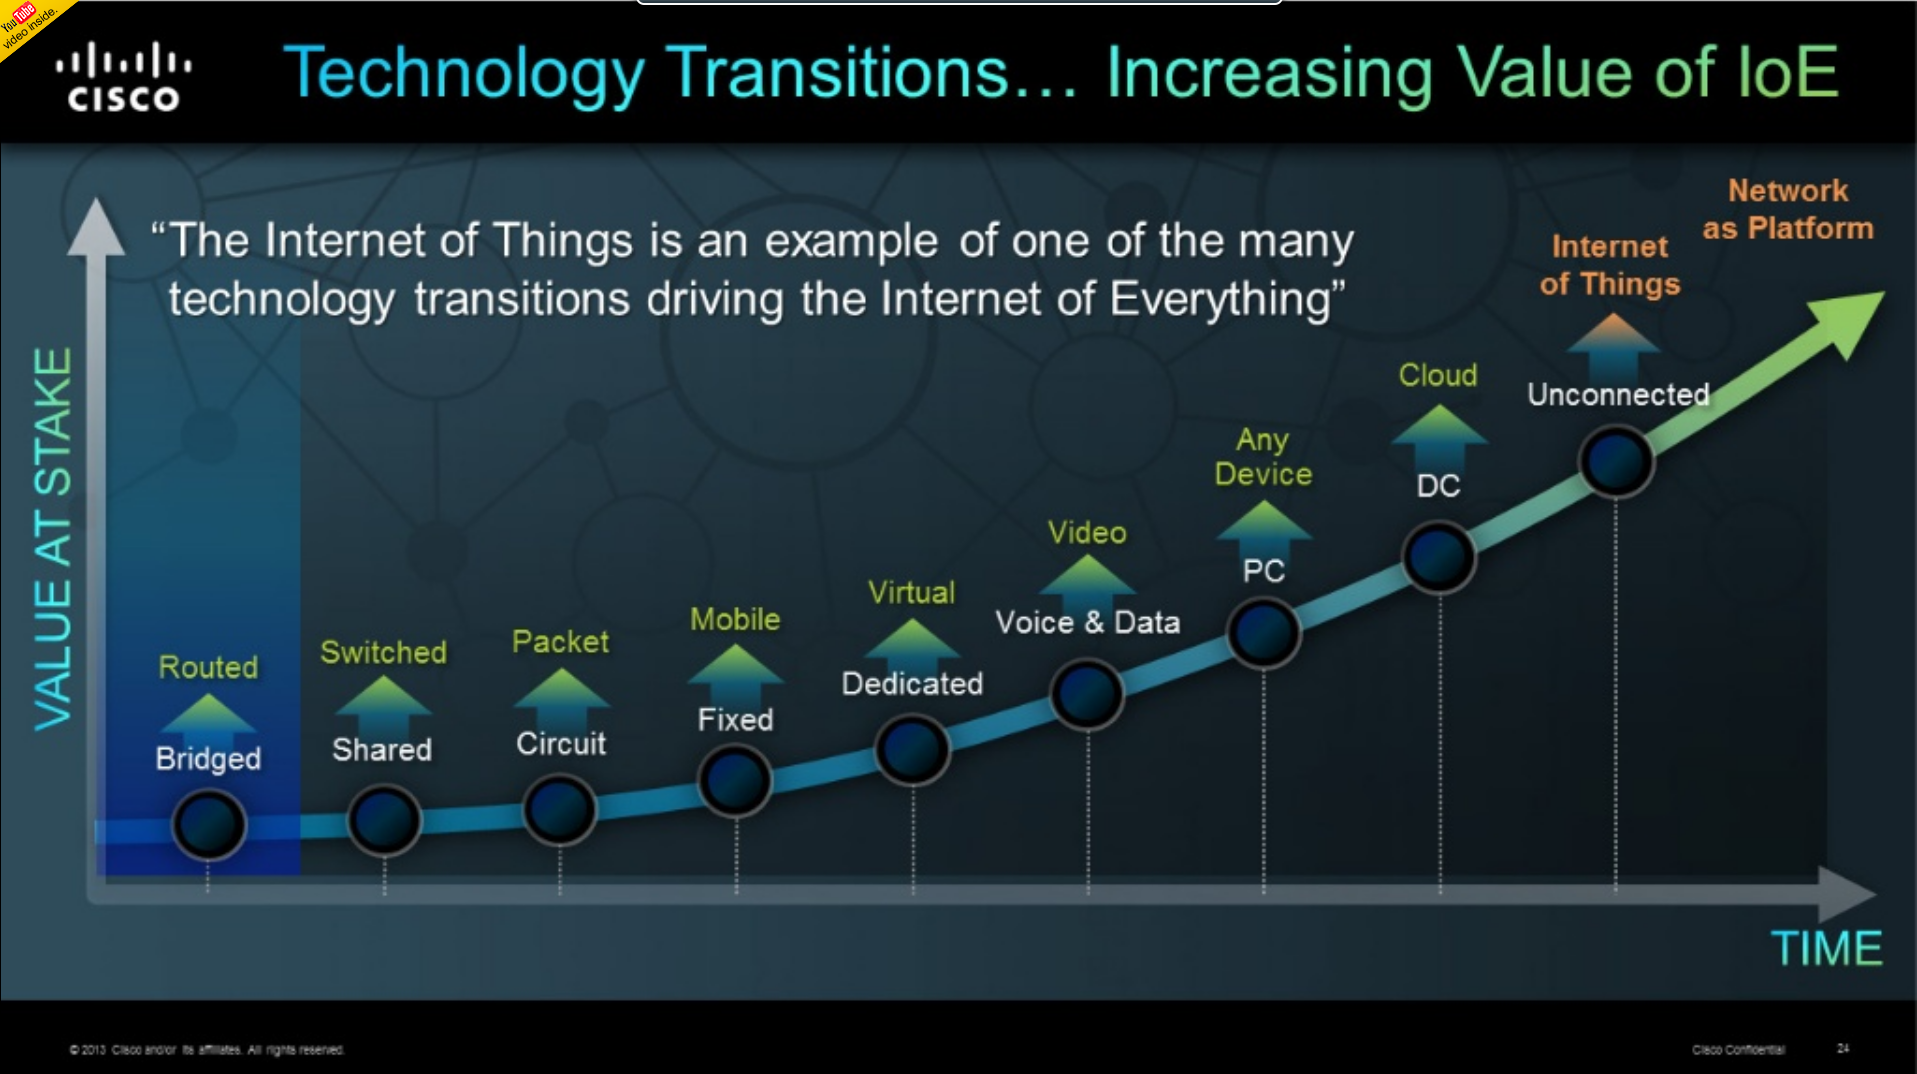
\includegraphics[width=11cm]{../pics/Cisco-tech-leading2IoE}
	\caption{Credit: \href{http://www.slideshare.net/Cisco/john-chambers-partner-summit-keynote}{John Chambers Keynote (Cisco, 2013)}}
	\end{figure}
}

\frame{
	\frametitle{The 4$^{th}$ Industrial Revolution}
	\framesubtitle{Emerging Technologies  (\href{http://www.gartner.com/technology/research/hype-cycles/}{Gartner's Hype Cycle}, 2015)}
	\begin{figure}
	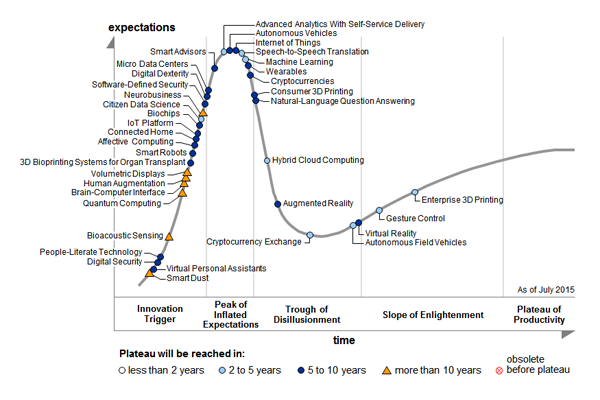
\includegraphics[width=11cm]{../pics/gartner2015_emerging-tech-hc}
	\end{figure}
}

\frame{
	\frametitle{The 4$^{th}$ Industrial Revolution}
	\framesubtitle{It's also the way we work, e.g. OT vs. IT}
	\begin{figure}
	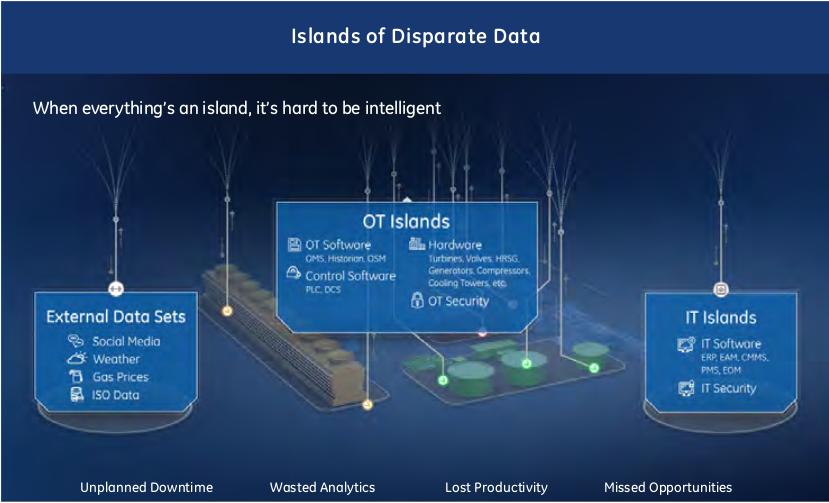
\includegraphics[width=11cm]{../pics/GE-OT-IT-data-islands}
	\caption{Credit: \href{http://go.digital.ge.com/IIOT-unlocking-business-value.html}{GE White Paper ``Unlocking Business Value through Industrial Data Management''}}
	\end{figure}
}

\frame{
	\frametitle{The 4$^{th}$ Industrial Revolution}
%	\framesubtitle{Cisco's estimates of the \href{http://ioeassessment.cisco.com/explore/full\#/country/can}{Value at Stake for Canada (2013)}}
	\framesubtitle{Estimation of the Value at Stake for Canada (\cite{ciscoVAT2013})}
	\begin{figure}
	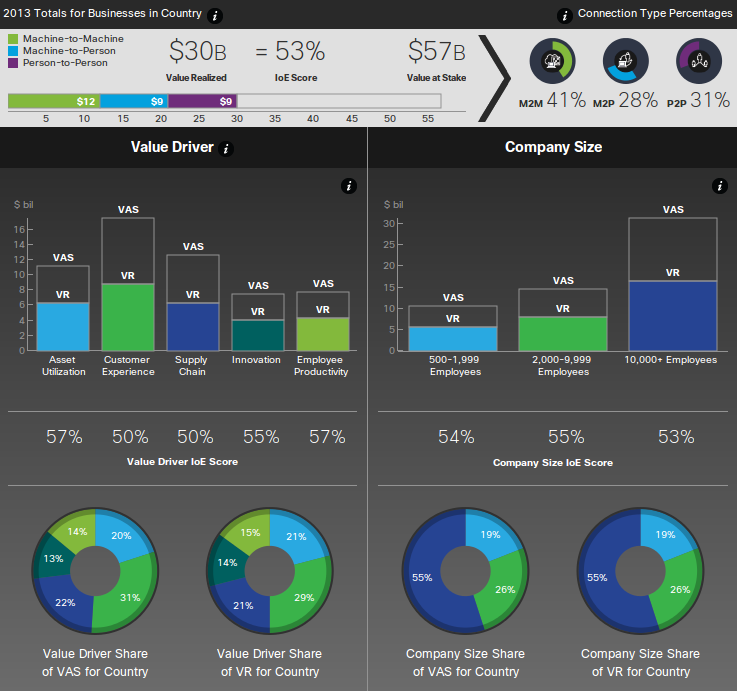
\includegraphics[height=7.5cm]{../pics/Cisco-IoE-Canada}
%	\caption{Credit: \href{http://ioeassessment.cisco.com/explore/full\#/country/can}{Cisco Value at Stake Study (2013)}}
	\end{figure}
}

\frame{
	\frametitle{The 4$^{th}$ Industrial Revolution}
	\framesubtitle{The market value (to be captured): \$19T over 10 years according to Cisco}
	\begin{figure}
	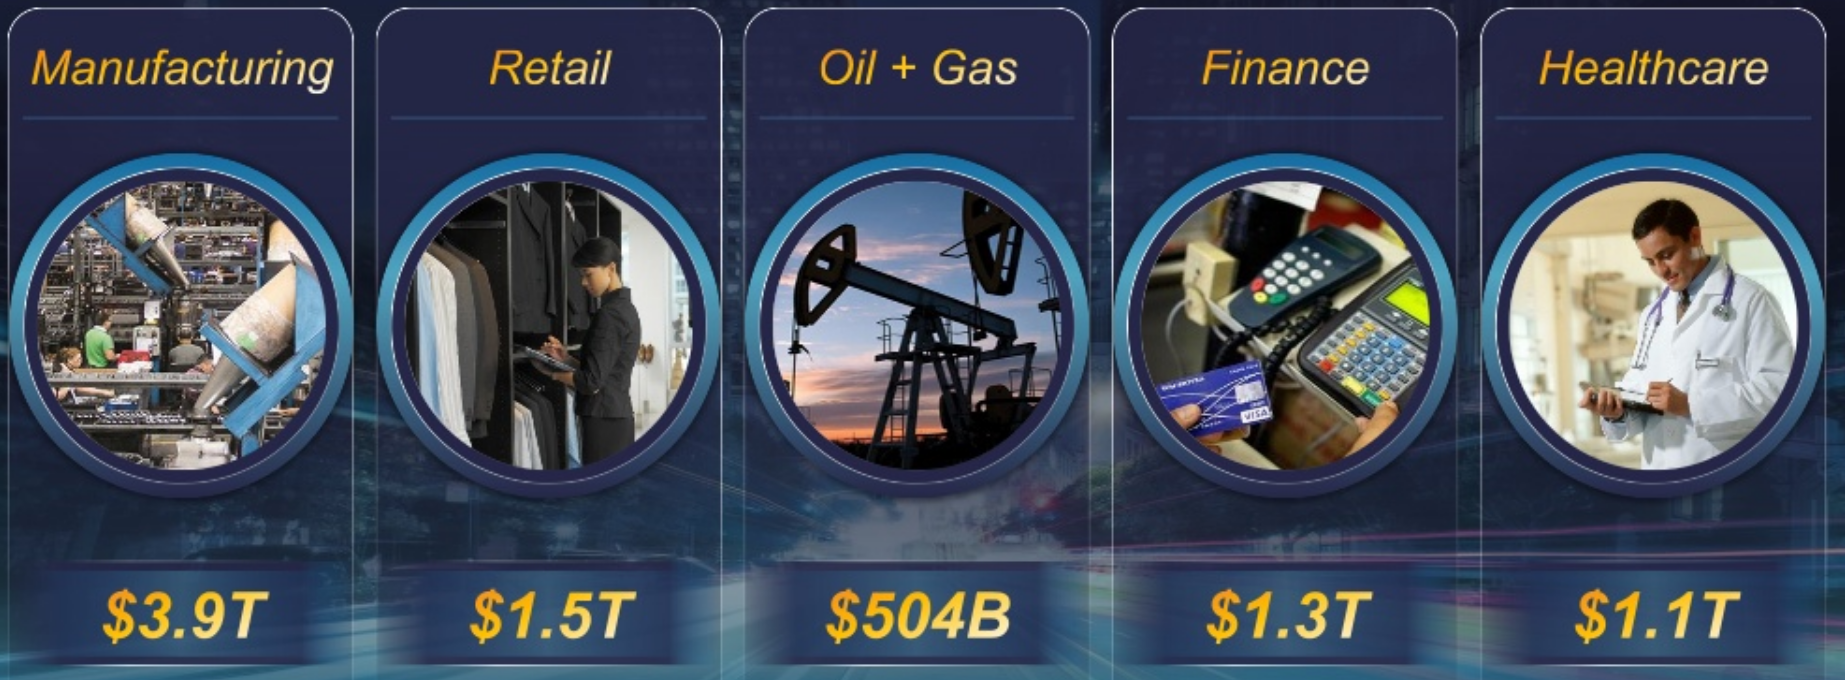
\includegraphics[width=11cm]{../pics/Cisco-IoE-main-verticals}
	\caption{Verticals with highest \$ potential Credit: \href{http://www.slideshare.net/Cisco/john-chambers-cisco-live-keynote-presentation}{John Chambers Keynote (Cisco, 2014)}}
	\end{figure}
}

\frame{
	\frametitle{The 4$^{th}$ Industrial Revolution}
	\framesubtitle{A sense of urgency \& the race for survival}
	\begin{figure}
	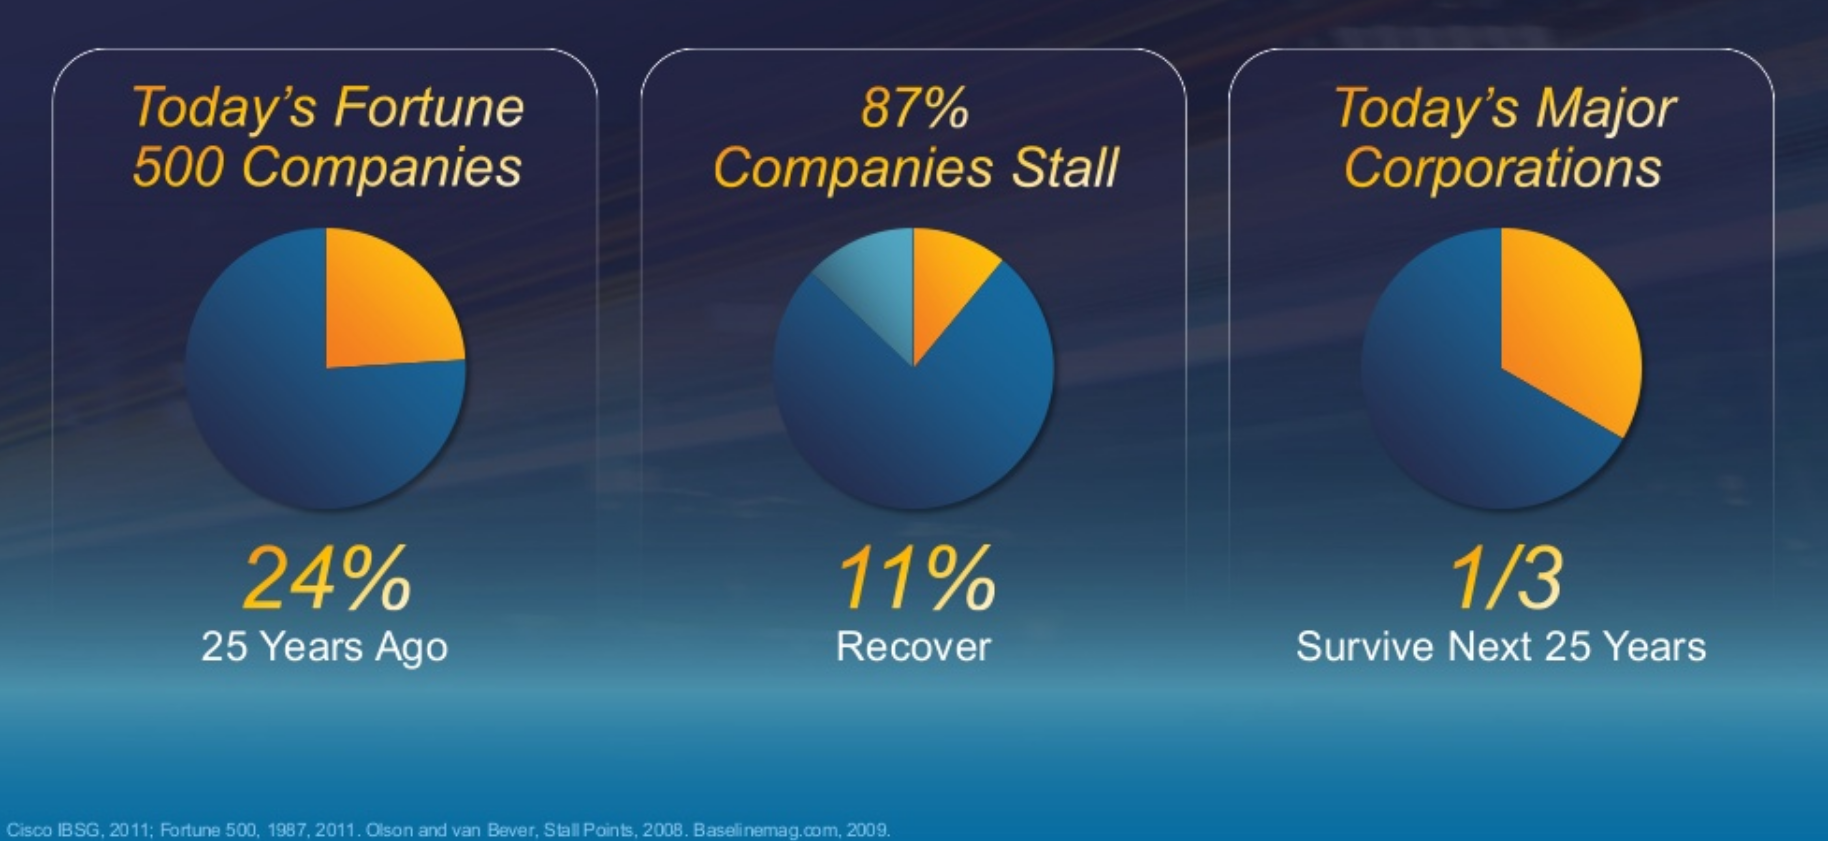
\includegraphics[width=11cm]{../pics/Cisco-Cie-survival-rate}
	\caption{Credit: \href{http://www.slideshare.net/Cisco/john-chambers-cisco-live-keynote-presentation}{John Chambers Keynote (Cisco, 2014)}}
	\end{figure}
}

\frame{
	\frametitle{The 4$^{th}$ Industrial Revolution}
	\framesubtitle{SWOT Analysis (Credit: Diagram by Xhienne [\href{http://creativecommons.org/licenses/by-sa/2.5}{CC BY-SA 2.5}], via Wikimedia Commons)}
	\begin{figure}
	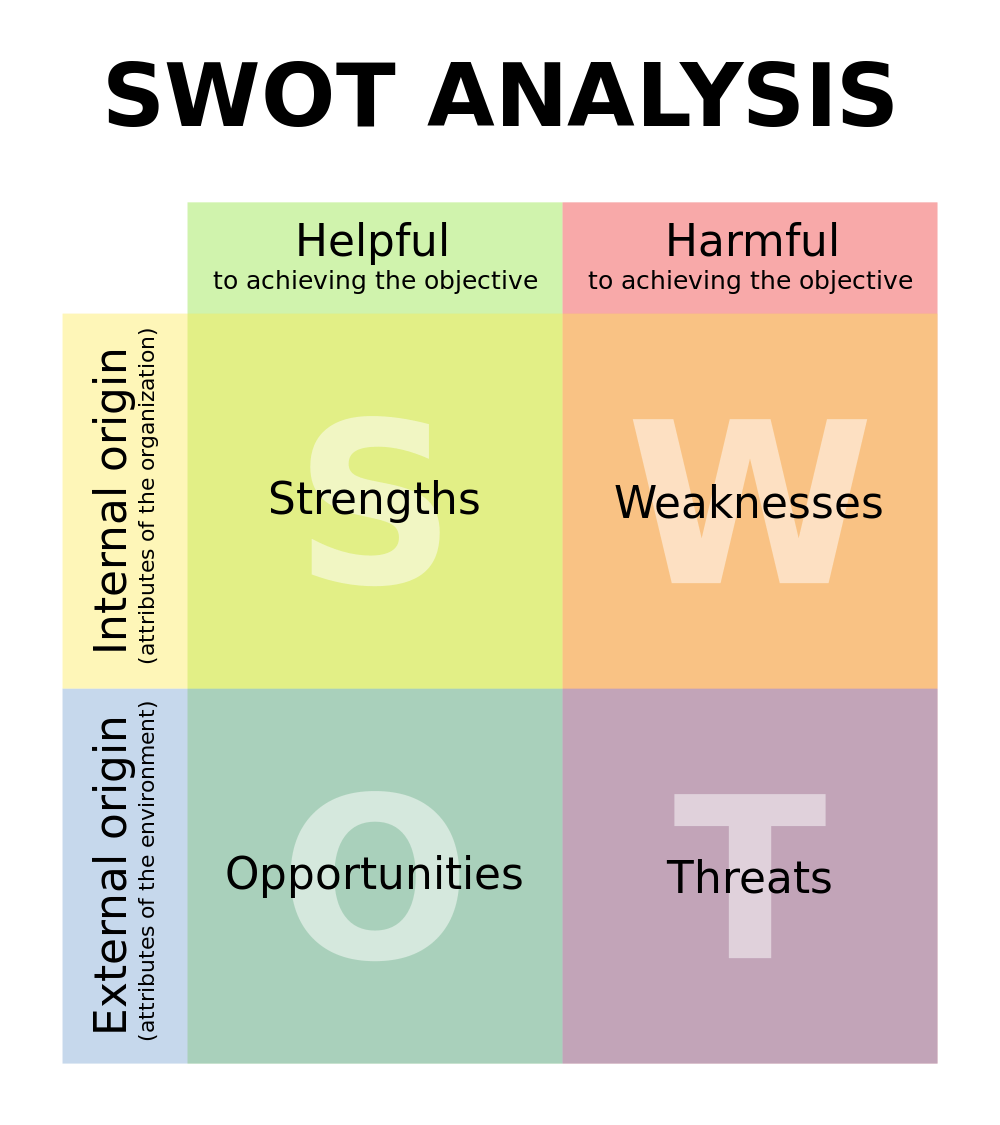
\includegraphics[height=7.5cm]{../pics/1000px-SWOT_en}
	\end{figure}
}

\frame{
	\frametitle{The 4$^{th}$ Industrial Revolution}
	\framesubtitle{Exercise}
	\begin{alertblock}{Group Work}
		Assess the situation for an Industry (or pick a particular company, e.g. your coop).
	\end{alertblock}
}

\frame{
	\frametitle{The 4$^{th}$ Industrial Revolution}
	\framesubtitle{References}
	% keyword refers to bib file: references-KEYWORD.bib, and to the Tex file: section-KEYWORD.tex
	\printbibliography[keyword=4th-industrial-revolution]
}

\frame{
	\frametitle{The 4$^{th}$ Industrial Revolution}
	\framesubtitle{}
}

%\frame{
%	\frametitle{The 4$^{th}$ Industrial Revolution}
%	\framesubtitle{References}
%	\begin{itemize}
%		\item \url{http://ioeassessment.cisco.com/} 
%	\end{itemize}
%}

